\chapter{\textit{Data Warehouse}} 
\label{chap:arquitetura}

Neste capítulo será apresentada a fundamentação teórica sobre \textit{Data Warehouse} e como utiliza-lo para o monitoramento de métricas. Também será apresentado o ambiente de \textit{Data Warehouse} utilizado na solução proposta por \citeonline{rego_monitoramento_2014}, no qual este trabalho busca analisar a eficácia e eficiência no monitoramento de métricas,  e como ela foi desenvolvida.  

\section{Definição}

Na década de 80 as organizações perceberam a importância de não apenas usar dados para propósitos operacionais, mas também para derivar a inteligência por trás deles. Essa inteligência não só justificaria as decisões passadas, mas também ajudaria na tomada de decisões para o futuro. O termo \textit{Business Intelligence} tornou-se cada vez mais popular, e foi durante o final dos anos 1980 que pesquisadores da IBM, Barry Devlin e Paul Murphy, desenvolveram o conceito de \textit{Business data warehouse }. A partir que aplicações de \textit{business intelligence } foram surgindo, foi rapidamente verificado que os dados de bancos transacionais tinham que primeiramente ser transformados e armazenados em outros bancos de dados com um esquema específico para poderem derivar de sua inteligência. Esta base de dados poderia ser usada para arquivamento, e seria maior em tamanho do que as bases de dados transacionais, mas seu \textit{design} seria ideal para executar relatórios que permitem as grandes organizações planejarem e tomarem decisões de forma proativa. Este banco de dados, normalmente armazenando as atividades realizadas no passado e no presente das organizações, foi chamado de \textit{Data Warehouse} \cite{neeraj_sharma_2011}.

Para \citeonline{Inmon2002}, \textit{Data Warehouse} é uma coleção de dados que tem como característica ser orientada a assunto, integrada, não volátil e temporal. Por orientação a assunto, podemos entender como um foco em algum aspecto específico da organização. O fato do ambiente ser integrado remete ao fato dele ser alimentado com dados que têm como origem múltiplas fontes, integrando esses dados de maneira a construir uma única orientação. Como um conjunto não volátil e temporal de dados, é entendido que a informação carregada remete a um determinado momento da aplicação, possibilitando assim acesso a diferentes intervalos de tempo, não havendo como modificá-los atualizando em tempo real.

Segundo \citeonline{andre2000},  \textit{Data Warehousing} é a infra-estrutura tecnológica de \textit{hardware} e \textit{software} para a atividade de análise gerencial. Agora que sabemos o que é o \textit{data wharehouse} e \textit{Data Warehousing}, serão mostrado os componentes que compõem um ambiente completo de \textit{data warehousing}. É importante entender como os componentes funcionam individualmente antes de começarem a ser combinados para se criar um \textit{data warehouse}. Cada componente do armazém tem uma função específica. É preciso aprender a importância estratégica de cada componente e como manuseá-los efetivamente para fazer uso do \textit{data warehousing}. Uma das maiores ameaças ao sucesso no \textit{data warehousing} é confundir os papéis e as funções dos componentes \cite{Kimball2002}. A Figura \ref{fig:etl} descreve uma arquitetura geral de um ambiente de \textit{Data Warehousing}, os componentes do ambiente serão esclarecidos no decorrer deste capítulo.

\begin{figure}[h!]
\centering
\includegraphics[keepaspectratio=false,scale=0.50]{figuras/figuras_nilton/etl.eps}
\caption{Arquitetura de um ambiente de Data Warehousing}
\label{fig:etl}
\end{figure}
\FloatBarrier


\section{\textit{Extraction-Transformation-Load}}

A \textit{Staging Area} é uma área de armazenamento onde acontece o processo de ETL. Na Figura \ref{fig:etl}, as etapas 1- Extração, 2- Transformação e 3- Carga formam o processo de \textit{Extraction-Transformation-Load} (ETL). Cada uma das etapas recebe a seguinte descrição:

\begin{easylist}[itemize]

	& \textbf{Extração: } Primeira etapa do processo de ETL, consiste na leitura e entendimento da fonte 		dos dados, copiando os que são necessários para futuros trabalhos \cite{Kimball2002}.  
	& \textbf{Transformação: } Após a etapa de extração ter sido feita, os dados podem receber diversos tipos de transformações, que incluem correções de conflitos, conversão de formatos, remoção de campos que não são úteis, combinação entre dados de diversas fontes, entre outros \cite{Kimball2002}.
	& \textbf{Carga: } Após ter sido realizado o processo de transformação, os dados já estão prontos para serem carregados no \textit{Data Warehouse}, tornando possível que todos os dados visualizados após esse processo reflitam a informação que passou pelos processos de extração e transformação \cite{neeraj_sharma_2011}.  

	\end{easylist}

\section{Modelagem Dimensional}

Modelagem dimensional é um novo nome para uma velha técnica para deixar os bancos de dados simples e compreensíveis. No início dos anos 70 as organizações de TI, consultores, usuários finais e fornecedores tiveram que migrar para uma estrutura dimensional simples que combinasse com a necessidade humana pela simplicidade \cite{Kimball2002}. 

Segundo \citeonline{Kimball2002}, a modelagem dimensional tem sido amplamente aceita como a técnica dominante para a apresentação do \textit{data warehouse}. Os profissionais e especialistas de \textit{data warehouse} reconhecem que a apresentação do \textit{data warehouse} deve ser fundamentada na simplicidade. A simplicidade é a chave fundamental que permite que os usuários entendam facilmente as bases de dados e naveguem de forma eficiente no bancos de dados do \textit{software}. 

Para facilitar na difusão do conceito de modelagem dimensional \citeonline{Kimball2002} utiliza como exemplo um diretor geral que descreve seus negócios  como "Nós vendemos produtos em várias áreas de negócio e medimos nosso desempenho ao longo do tempo". Assim, designers dimensionais colocariam em ênfase o produto, as áreas de negócio e o tempo, pensando intuitivamente neste negócio como um cubo de dados, onde as bordas estariam marcadas como produto, negócio e tempo. Pontos dentro do cubo são onde as medições que combinam produtos, áreas de negócio e tempo são salvas. A capacidade de visualizar algo tão abstrato como um conjunto de dados de uma forma concreta e tangível é o segredo da compreensão.

Os conceitos básicos da modelagem dimensional são: fatos, dimensões e medidas. Um fato é uma coleção de itens de dados relacionados, que consiste em medidas e dados de contexto. Ele representa tipicamente itens de negócios ou transações de negócio. A dimensão é uma coleção de dados que descrevem uma dimensão negócio. Dimensões determinam o contextual a fundo para os fatos; eles são os parâmetros nos quais queremos realizar a \textit{On-Line Analytic Processing (OLAP)}. A medida é um atributo numérico de um fato, que representa o desempenho ou comportamento do negócio em relação às dimensões \cite{marotta2000}.

Considerando o contexto relacional, existem dois modelos básicos que são utilizados na modelagem dimensional: modelo de estrela e modelo de floco de neve. O modelo estrela é a estrutura básica de um modelo dimensional. Ele tem uma grande tabela central (tabelas fato) e um conjunto de pequenas tabelas (tabelas dimensão) dispostos em um padrão radial 
ao redor da tabela central, como é mostrado na Figura \ref{fig:estrela}. O modelo de floco de neve é o resultado da decomposição de uma ou mais das dimensões \cite{marotta2000}.
 
\begin{figure}[h!]
\centering
\includegraphics[keepaspectratio=false,scale=0.50]{figuras/figuras_nilton/star.eps}
\caption{Esquema estrela extraído de \citeonline{valeria2012}}
\label{fig:estrela}
\end{figure}
\FloatBarrier
 
\subsection{OLAP \textit{(On-Line Analytic Processing)}}

A atividade que consiste em buscar e apresentar os dados de um \textit{Data Warehouse}, sendo essa busca quase sempre baseada em um cubo multidimensional de dados, é chamada de \textit{On-Line Analytic Processing} (OLAP) \cite{Kimball2002}. Segundo \citeonline{neeraj_sharma_2011}, \textit{On-Line Analytic Processing(OLAP)} refere-se a cargas onde grandes quantidades de históricos de dados são processados para gerar relatórios e executar análise de dados. Normalmente, bancos de dados que utilizam OLAP são alimentados a partir de bancos de dados \textit{On-Line Transaction Processing} (OLTP) que são alterados para gerir cargas OLAP. Um banco de dados OLAP armazena um grande volume com os mesmos dados transacionais que um banco de dados OLTP, mas estes dados são transformados pelo processo de ETL para permitir um melhor desempenho para geração de relatórios e para facilitar as análises. Geralmente sistemas OLTP são ajustados para inserções, atualizações e exclusões bem rápidas, enquanto os sistemas OLAP estão ajustados para consultas rápidas.

A tabela \ref{tab:hilmer} evidencia as diferenças entre aplicações OLTP e OLAP extraídas do trabalho de \cite{hilmer2002}: 

\begin{table}[!ht]
	\begin{center}
	
	\input{tabelas/tabelasNilton/hilmer_olap_oltp.ltx} 
	\caption{Diferenças entre OLTP e OLAP extraídas de \citeonline{hilmer2002}}
	\label{tab:hilmer}
	\end{center}
	\end{table}	
	\FloatBarrier
	
	
No modelo multidimensional, os dados são organizados em múltiplas dimensões, e cada dimensão contém vários níveis de abstração definidos pelas hierarquias. Esta organização fornece aos usuários a flexibilidade para visualizar os dados a partir de diferentes perspectivas. Existe uma série de operações de cubo de dados OLAP para materializar esses diferentes pontos de vista, permitindo consultas interativas e análises de dados. Assim, OLAP fornece um ambiente amigável para análise de dados interativos.

Entre as operações OLAP estão:	


\begin{easylist}[itemize]

	& \textbf{\textit{Drill Down:}} Busca aumentar o nível de detalhamento, partindo de um certo nível de dados para um nível mais detalhado \cite{neeraj_sharma_2011}.  
	
	& \textbf{\textit{Drill Up:}} Ao contrário da operação \textit{Drill Down}, a \textit{Roll Up} parte de um nível mais detalhado para um nível menos detalhado  \cite{neeraj_sharma_2011}.\\
	
	
	\begin{figure}[h!]
\centering
\includegraphics[keepaspectratio=false,scale=1.3]{figuras/figuras_nilton/drillDownUp.eps}
\caption{Exemplo de operações \textit{Drill Down}(direita) e \textit{Drill up}(esquerda) extraídos de \citeonline{golfarelli_data_2009}}
\label{fig:drillUpDown}
\end{figure}
\FloatBarrier
	
	& \textbf{\textit{Slice and Dice:}} Técnica com filosofia parecida à cláusula \textit{where} usada em \textit{SQL}. Permite que sejam criadas restrições na análise dos dados \cite{valeria2012}. O \textit{Slice} faz restrição de um valor ao longo de uma dimensão, já o \textit{Dice} faz restrições de valores em várias dimensões. Semelhante ao \textit{Slice}, só que mais complexo.\\
	
	
		\begin{figure}[h!]
\centering

\includegraphics[keepaspectratio=false,scale=2.0]{figuras/figuras_nilton/sliceDice.eps}
\caption{Exemplo de operações \textit{Slice}(acima) e \textit{Dice}(embaixo) extraídos de \citeonline{golfarelli_data_2009}}
\label{fig:sliceDice}
\end{figure}
\FloatBarrier
	
	& \textbf{\textit{Drill Across:}} Permite que diferentes cubos sejam concatenados \cite{hilmer2002}. Uma operação do tipo \textit{Drill Across} irá simplesmente unir diferentes tabelas fato através de dimensões correspondentes \cite{kimball1998data}.\\
	 
	
			\begin{figure}[h!]
\centering
\includegraphics[keepaspectratio=false,scale=2.0]{figuras/figuras_nilton/drilAcross.eps}
\caption{Exemplo da operação \textit{Drill Across} extraído de \citeonline{golfarelli_data_2009}}
\label{fig:drillAcross}
\end{figure}
\FloatBarrier
	
	& \textbf{\textit{Pivoting:}} Metaforicamente, significa rotacionar o cubo. Essa técnica altera a ordenação das tabelas dimensionais \cite{hilmer2002}.\\
	 
	
				\begin{figure}[h!]
\centering
\includegraphics[keepaspectratio=false,scale=2.0]{figuras/figuras_nilton/pivoting.eps}
\caption{Exemplo da operação \textit{Pivoting} extraído de \citeonline{golfarelli_data_2009}}
\label{fig:pivoting}
\end{figure}
\FloatBarrier
	
	\end{easylist}
	
\section{Ambiente de \textit{Data Warehousing} para Métricas de Código-Fonte}


Para a implementação do ambiente de Data Warehousing para métricas de código-
fonte, \citeonline{rego_monitoramento_2014} definiu a arquitetura tal como mostra na Figura \ref{fig:etl}.

A ferramenta de análise estática de código-fonte escolhida por \citeonline{rego_monitoramento_2014} foi a Analizo. A Analizo  possibilita emitir saídas das métricas em CSV que detalham nome da classe e as respectivas métricas, o que permitiu a seu trabalho incorporar a análise das métricas ANPM, AMLOC, CBO, NPA.

\citeonline{rego_monitoramento_2014} seguiu a metodologia de \cite{Kimball2002}, apresentada na Figura \ref{fig:metodologia-dw}, para o seu projeto de \textit{data warehouse}. Seguindo esta metodologia, \citeonline{rego_monitoramento_2014} definiu os seguintes requisitos de negócio que a sua solução deveria suportar:

\begin{easylist}[itemize]

	& \textbf{Requisito 1:} Visualizar o intervalo qualitativo obtido para cada métrica de código-fonte em uma determinada \textit{release} do projeto para a configuração O\textit{pen JDK8 Metrics}.
	 
	& \textbf{Requisito 2:} Comparar o intervalo qualitativo obtido para cada métrica de código-fonte ao longo de todas as \textit{releases} de um projeto para a configuração \textit{Open JDK8 Metrics}.

	& \textbf{Requisito 3:} Visualizar o valor percentil obtido para cada métrica de código-fonte em uma determinada \textit{release} do projeto para a configuração \textit{Open JDK8 Metrics}.
	
	& \textbf{Requisito 4:} Comparar o valor percentil de cada métrica de código-fonte ao longo de todas as \textit{releases} para a configuração \textit{Open JDK8 Metrics}.
	
	& \textbf{Requisito 5:} Visualizar o intervalo qualitativo obtido para cada métrica de código-fonte em uma determinada \textit{release} do projeto para a configuração \textit{Tomcat Metrics}.
	
	& \textbf{Requisito 6:} Comparar o intervalo qualitativo obtido para cada métrica de código-fonte ao longo de todas as \textit{releases} de um projeto para a configuração \textit{Tomcat Metrics}.
	
	& \textbf{Requisito 7:} Visualizar a medida obtida para cada métrica de código-fonte em uma determinada \textit{release }do projeto para a configuração \textit{Tomcat Metrics}.
	
	& \textbf{Requisito 8:} Comparar o valor percentil obtido para cada métrica de código-fonte ao longo de todas as \textit{releases} para a configuração \textit{Tomcat Metrics}.
	
	& \textbf{Requisito 9:} Visualizar a quantidade de cenários de limpeza identificados por tipo de cenários de limpeza de código-fonte em cada classe ao longo de cada \textit{release} de um projeto.
	
	& \textbf{Requisito 10:} Comparar a quantidade de cenários de limpeza por tipo de cenários de limpeza de código-fonte em uma \textit{release} de um projeto.
	
	& \textbf{Requisito 11:} Visualizar o total de cenários de limpeza em uma determinada \textit{release} de um projeto.
	
	& \textbf{Requisito 12:} Visualizar cada uma das classes com um determinado cenário de limpeza de código-fonte ao longo das \textit{releases} do projeto.
	
	& \textbf{Requisito 13:} Visualizar as 10 classes de um projeto com menor número de cenários de limpeza identificados.
	
	& \textbf{Requisito 14:} Visualizar as 10 classes de um projeto com maior número de cenários de limpeza identificados.
	
	& \textbf{Requisito 15:} Acompanhar a Taxa de Aproveitamento de Oportunidades de Melhoria de Código-Fonte que é a divisão do total de cenários de limpeza identificados em uma \textit{release} e o o número total de classes da mesma \textit{release} de um projeto

	\end{easylist}

\begin{figure}[ht!]
\centering
\includegraphics[keepaspectratio=true,scale=0.19]{figuras/figuras_nilton/metodologiaKimball.eps}
\caption{Metodologia de Projeto de \textit{Data Warehouse} proposta por \citeonline{Kimball2002} extraída de \citeonline{rego_monitoramento_2014} }
\label{fig:metodologia-dw}
\end{figure}
\FloatBarrier

	
Ainda seguindo a metodologia de \cite{Kimball2002}, \citeonline{rego_monitoramento_2014} identificou fatos e dimensões no contexto de monitoramento de métricas, como mostra a Tabela \ref{tab:fatos-dimensoes}

\begin{table}[!ht]
	\begin{center}
	
	\input{tabelas/tabelasNilton/fatos-dimensoes.ltx} 
	\caption{Fatos e dimensões identificadas por \citeonline{rego_monitoramento_2014}}
	\label{tab:fatos-dimensoes}
	\end{center}
	\end{table}	
	\FloatBarrier


Após a identificação dos fatos e das dimensões, \citeonline{rego_monitoramento_2014} construiu o projeto físico do \textit{Data Warehouse} que pode ser visto na Figura \ref{fig:arquitetura_solucao}. A Tabela \ref{tab:tabelas-fatos-dimensoes} facilita a interpretação do projeto físico.

\begin{figure}[h!]
\centering
\includegraphics[keepaspectratio=false,scale=0.50]{figuras/figuras_nilton/modelo-dw-baufaker.eps}
\caption{Projeto físico do \textit{Data Warehouse} extraído de \citeonline{rego_monitoramento_2014}}
\label{fig:arquitetura_solucao}
\end{figure}
\FloatBarrier

\begin{table}[!ht]
	\begin{center}
	
	\input{tabelas/tabelasNilton/tabelas-fatos-tabelas-dimensoes.ltx} 
	\caption{Tabelas fatos e tabelas dimensões elaboradas por \citeonline{rego_monitoramento_2014}}
	\label{tab:tabelas-fatos-dimensoes}
	\end{center}
	\end{table}	
	\FloatBarrier
	
Visando facilitar o processo de ETL principalmente na etapa da transformação, \citeonline{rego_monitoramento_2014} criou uma área de metadados mostrada na Figura \ref{fig:metadados} com intuito de tratar os dados que representam os próprios dados dos processos de negócio. A Tabela \ref{tab:tabelasMetadadosDescricao} descreve as tabelas contidas na área de metadados do \textit{Data Warehouse}.

\begin{figure}[h!]
\centering
\includegraphics[keepaspectratio=false,scale=0.6]{figuras/figuras_nilton/metadados-baufaker.eps}
\caption{Projeto físico do \textit{Data Warehouse} extraído de \citeonline{rego_monitoramento_2014}}
\label{fig:metadados}
\end{figure}
\FloatBarrier

\begin{table}[!ht]
	\begin{center}
	
	\input{tabelas/tabelasNilton/tabelaMetadadosDescricao.ltx} 
	\caption{Descrição das Tabelas do Metadados do \textit{Data Warehouse} }
	\label{tab:tabelasMetadadosDescricao}
	\end{center}
	\end{table}	
	\FloatBarrier

\subsection{Ferramentas de \textit{Data Warehousing}}
\label{ferramentas}

Entre as alternativas de código aberto que suportam um modelo dimensional, \citeonline{rego_monitoramento_2014}  utilizou o \textit{Pentaho Business Analytics Community Edition}. Esta alternativa livre apresenta soluções que cobrem as áreas de ETL, \textit{reporting}, \textit{OLAP} e mineração de dados. A Figura \ref{fig:arquiteturaAmbiente}, apresenta o modo como cada uma das ferramentas está disposta na arquitetura do ambiente de \textit{Data Warehousing} para Métricas de Código-Fonte.

Segue abaixo as ferramentas utilizadas em cada etapa do \textit{Data Warehouse}:

\begin{easylist}[itemize]

	& \textbf{ETL:} Pentaho Data Integration Community Edition ou Kettle.
	 
	& \textbf{Implementação das Consultas OLAP e Visualização de Dados:} \textit{Pentaho BI Platform 8}, provê uma arquitetura e a infraestrutura para soluções de \textit{Business Inteligence}, \textit{Data Mining} e a camada de visualização de dados do \textit{Data Warehouse}. Junto ao \textit{Pentaho BI Platform 8} foi utilizado o \textit{plugin Saiku Analytics} que oferece serviços de apoio a operações OLAP e à visualização de dados. Na arquitetura do \textit{Saiku Analytics}, está incorporado outro software livre que realiza consulta, chamado de \textit{Mondrian OLAP}. 
	
	& \textbf{Análise estática de código-fonte:}\textit{Analizo}, possibilita emitir saídas das métricas em CSV que detalham o nome da classe e as suas respectivas métrica.

	\end{easylist}
	
	\begin{figure}[h!]
\centering
\includegraphics[keepaspectratio=false,scale=0.2]{figuras/figuras_nilton/pentaho-tools.eps}
\caption{Arquitetura Ambiente de \textit{Data Warehousing} para Métricas de Código-Fonte extraído de \citeonline{rego_monitoramento_2014}}
\label{fig:arquiteturaAmbiente}
\end{figure}
\FloatBarrier

\section{Considerações finais do capítulo}

Nesse capítulo foi apresentada a solução proposta no trabalho de \citeonline{rego_monitoramento_2014}, bem como a base teórica para sua compreensão. No próximo capítulo será apresentado o projeto de estudo de caso que visa a análise da eficácia e eficiência da solução de DW proposta nesse capítulo.
